% Basis for V_2 (blue) and Haar wavelets basis for W_2 (red)
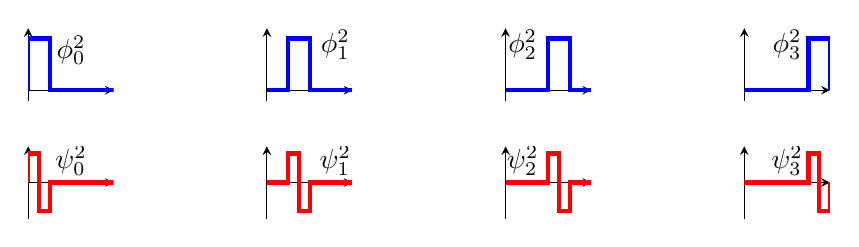
\begin{tikzpicture}
  % V_2 Scaling functions (row above)
  % Scaling function 1: [0, 1/4)
  \begin{axis}[
    at={(0,1.5cm)},
    width=0.22\textwidth,
    height=2.5cm,
    xmin=0, xmax=1,
    ymin=-0.2, ymax=1.2,
    ytick=\empty,
    xtick=\empty,
    axis x line=middle,
    axis y line=center,
  ]
    \addplot[const plot, line width=1.5pt, color=blue] coordinates {
      (0,0) (0,1) (0.25,1) (0.25,0) (1,0)
    };
    \node[above] at (0.5, 0.3) {$\phi_0^2$};
  \end{axis}
  % Scaling function 2: [1/4, 1/2)
  \begin{axis}[
    at={(0.25\textwidth,1.5cm)},
    width=0.22\textwidth,
    height=2.5cm,
    xmin=0, xmax=1,
    ymin=-0.2, ymax=1.2,
    ytick=\empty,
    xtick=\empty,
    axis x line=middle,
    axis y line=center,
  ]
    \addplot[const plot, line width=1.5pt, color=blue] coordinates {
      (0,0) (0.25,0) (0.25,1) (0.5,1) (0.5,0) (1,0)
    };
    \node[above] at (0.8, 0.4) {$\phi_1^2$};
  \end{axis}
  % Scaling function 3: [1/2, 3/4)
  \begin{axis}[
    at={(0.5\textwidth,1.5cm)},
    width=0.22\textwidth,
    height=2.5cm,
    xmin=0, xmax=1,
    ymin=-0.2, ymax=1.2,
    ytick=\empty,
    xtick=\empty,
    axis x line=middle,
    axis y line=center,
  ]
    \addplot[const plot, line width=1.5pt, color=blue] coordinates {
      (0,0) (0.5,0) (0.5,1) (0.75,1) (0.75,0) (1,0)
    };
    \node[above] at (0.2, 0.4) {$\phi_2^2$};
  \end{axis}
  % Scaling function 4: [3/4, 1)
  \begin{axis}[
    at={(0.75\textwidth,1.5cm)},
    width=0.22\textwidth,
    height=2.5cm,
    xmin=0, xmax=1,
    ymin=-0.2, ymax=1.2,
    ytick=\empty,
    xtick=\empty,
    axis x line=middle,
    axis y line=center,
  ]
    \addplot[const plot, line width=1.5pt, color=blue] coordinates {
      (0,0) (0.75,0) (0.75,1) (1,1) (1,0)
    };
    \node[above] at (0.5, 0.4) {$\phi_3^2$};
  \end{axis}
  
  % Wavelet level 2, first: [0, 1/8) vs [1/8, 1/4)
  \begin{axis}[
    at={(0,0)},
    width=0.22\textwidth,
    height=2.5cm,
    xmin=0, xmax=1,
    ymin=-2.5, ymax=2.5,
    ytick=\empty,
    xtick=\empty,
    axis x line=middle,
    axis y line=center,
  ]
    \addplot[const plot, line width=1.5pt, color=red] coordinates {
      (0,0) (0,2) (0.125,2) (0.125,-2) (0.25,-2) (0.25,0) (1,0)
    };
    \node[above] at (0.5, -0.2) {$\psi_0^2$};
  \end{axis}
  % Wavelet level 2, second: [1/4, 3/8) vs [3/8, 1/2)
  \begin{axis}[
    at={(0.25\textwidth,0)},
    width=0.22\textwidth,
    height=2.5cm,
    xmin=0, xmax=1,
    ymin=-2.5, ymax=2.5,
    ytick=\empty,
    xtick=\empty,
    axis x line=middle,
    axis y line=center,
  ]
    \addplot[const plot, line width=1.5pt, color=red] coordinates {
      (0,0) (0.25,0) (0.25,2) (0.375,2) (0.375,-2) (0.5,-2) (0.5,0) (1,0)
    };
    \node[above] at (0.8, -0.2) {$\psi_1^2$};
  \end{axis}
  % Wavelet level 2, third: [1/2, 5/8) vs [5/8, 3/4)
  \begin{axis}[
    at={(0.5\textwidth,0)},
    width=0.22\textwidth,
    height=2.5cm,
    xmin=0, xmax=1,
    ymin=-2.5, ymax=2.5,
    ytick=\empty,
    xtick=\empty,
    axis x line=middle,
    axis y line=center,
  ]
    \addplot[const plot, line width=1.5pt, color=red] coordinates {
      (0,0) (0.5,0) (0.5,2) (0.625,2) (0.625,-2) (0.75,-2) (0.75,0) (1,0)
    };
    \node[above] at (0.2, -0.2) {$\psi_2^2$};
  \end{axis}
  % Wavelet level 2, fourth: [3/4, 7/8) vs [7/8, 1)
  \begin{axis}[
    at={(0.75\textwidth,0)},
    width=0.22\textwidth,
    height=2.5cm,
    xmin=0, xmax=1,
    ymin=-2.5, ymax=2.5,
    ytick=\empty,
    xtick=\empty,
    axis x line=middle,
    axis y line=center,
  ]
    \addplot[const plot, line width=1.5pt, color=red] coordinates {
      (0,0) (0.75,0) (0.75,2) (0.875,2) (0.875,-2) (1,-2) (1,0)
    };
    \node[above] at (0.5, -0.2) {$\psi_3^2$};
  \end{axis}
\end{tikzpicture}

